% ======================================================================
%  Tesis 1 · Ruta 1 — versión IEEE (LaTeX, clase IEEEtran)
%  Compilar con:  ./compilar.sh   (o latexmk -pdf main.tex)
%  Requiere TeX Live con la clase IEEEtran (paquete `ieeetran`) y `booktabs`.
% ======================================================================
\documentclass[conference]{IEEEtran}

\usepackage[utf8]{inputenc}
\usepackage[T1]{fontenc}
% babel en español si está instalado (paquete texlive-lang-spanish); si no, se compila igual
% en inglés y no se rompe la compilación.
\IfFileExists{spanish.ldf}{%
  \usepackage[spanish,es-tabla]{babel}%
}{%
  \usepackage[english]{babel}%
}
\usepackage{graphicx}
\usepackage{booktabs}
\usepackage{array}
\usepackage{amsmath,amssymb}
\usepackage{url}
\usepackage{microtype}
\usepackage{cite}
\usepackage[hidelinks]{hyperref}
\usepackage{xurl}

% Menos cajas desbordadas en columnas estrechas (IEEE es a dos columnas).
\setlength{\emergencystretch}{3em}
\tolerance=3000

\graphicspath{{../figures/}}

\begin{document}

\title{Metrología y transferencia del campo \texttt{confidence}\\
en modelos de decisión de pesos abiertos tipo Jev}

\author{%
\IEEEauthorblockN{Arbués Enrique Pérez Villegas}
\IEEEauthorblockA{Facultad de Ciencias\\
Universidad Nacional de Ingeniería (FC-UNI)\\
Lima, Perú\\
arbues.perez.v@uni.pe\\
ORCID: 0009-0004-7605-6569}
}

\maketitle

\begin{abstract}
Los modelos de decisión tipo Jev no generan texto: terminan la inferencia con un
\emph{readout} de logits y exponen un campo \texttt{confidence} sobre el que el ecosistema
fija umbrales de actuación. Sin embargo, el mismo nombre cubre definiciones
matemáticamente incompatibles. Este trabajo construye y publica un \emph{instrumento} para
medirlo: la especificación formal de las definiciones en uso, la librería
\texttt{jev-conf-\allowbreak metrics}, un conjunto de 65\,185 decisiones medidas sobre pesos abiertos y
una matriz de transferencia de umbrales que se regenera con un solo comando. Sobre 3\,564
celdas y 23 grupos (Laya en tres \emph{checkpoints}, Kev-0.8B y un control crudo), la
diferencia entre la definición más alta y la más baja de la \emph{misma} distribución tiene
mediana 0.288; el porte directo de un umbral se equivoca del orden de cien veces más que el
porte con el mapa cerrado cuando este existe; solo dos pares de definiciones transfieren por
identidad matemática; y la incompatibilidad es un fenómeno de $n \ge 3$. El mismo modelo
ofrece un ECE de 0.216 o de 0.577 según la definición. La contribución no es el hallazgo
sino el instrumento: sobrevive a él y mide cualquier implementación futura.
\end{abstract}

\begin{IEEEkeywords}
calibración, modelos de decisión, Jev, transferencia de umbrales, predicción selectiva,
pesos abiertos.
\end{IEEEkeywords}

\section{Introducción}
\label{sec:introduccion}

Los modelos de lenguaje grandes responden generando texto: la secuencia de tokens \emph{es} la respuesta y
su longitud es el costo. En septiembre de 2026 apareció una familia distinta. Los \textbf{modelos de
decisión} (o modelos \emph{System One}) reciben una pregunta y un conjunto \textbf{cerrado y etiquetado} de
opciones, y responden con \textbf{una opción y una probabilidad}, sin emitir texto: terminan la inferencia
con un \emph{readout} de logits en la posición de cada etiqueta permitida \cite{jev2026blog,jev2026docs}.
Su costo de salida es nulo ---el proveedor no cobra los tokens de salida---, su latencia es de decenas de milisegundos, y
se ofrecen como el componente que decide \guillemotleft qué hacer\guillemotright{} dentro de un sistema
mayor: clasificar, enrutar, verificar, abstenerse.

Jev, de TypeSafe, abrió la categoría el 18 de septiembre de 2026 \cite{jev2026blog}. En menos de un mes
floreció un ecosistema \textbf{open-source} de pesos abiertos que replica su contrato: \textbf{Laya} (421M,
la única implementación que publica el bucle de entrenamiento RLCD completo) \cite{layaRepo}, \textbf{Kev}
como familia entrenable \cite{kevRepo}, y una decena de derivados (Nimble, SemIf, Jeff, jev-lite, AnyJev,
entre otros) \cite{nimble,semif,jeff,jevLite,anyjev}. Todos exponen el mismo campo:
\textbf{\texttt{confidence}}.

Ese campo es el que hace útil al modelo. Un despliegue típico no usa la etiqueta a secas: fija un
\textbf{umbral} sobre \texttt{confidence} y decide \emph{actuar}, o \emph{escalar a un humano} cuando el
modelo no está seguro \cite{chow1970,geifman2017}. El umbral, por tanto, \textbf{es} la política. Y aquí
está el problema: aunque el campo se llame igual en todo el ecosistema, \textbf{su definición no es la
misma}.

\begin{table}[t]
\centering
\caption{Definiciones de \texttt{confidence} presentes en el ecosistema.}
\label{tab:definiciones}
\footnotesize
\resizebox{\columnwidth}{!}{%
\begin{tabular}{@{}lll@{}}
\toprule
implementación & definición de \texttt{confidence} & fórmula \\
\midrule
Jev & concentración & $(n\,p_{\max} - 1)/(n - 1)$ \cite{jev2026docs} \\
Laya (\texttt{choice}, \texttt{score}) & entropía normalizada & $1 - H(p)/\log n$ \cite{layastudio} \\
Laya (\texttt{noul}) & probabilidad binaria & $\max(p, 1 - p)$ \cite{layastudio} \\
jev-lite, Laya \texttt{answer\_confidence} & probabilidad ganadora & $p_{\max}$ \cite{jevLite} \\
otros derivados & margen, prior aprendido & $p_{(1)} - p_{(2)}$, \dots \\
\bottomrule
\end{tabular}}
\end{table}

El efecto es inmediato: una sola distribución sobre tres opciones, $(0.0118, 0.4629, 0.5253)$, produce
\textbf{tres valores distintos} de \texttt{confidence}: 0.288 con la fórmula de Jev, 0.3199 con la entropía
de Laya y 0.5253 con $p_{\max}$ \cite{rohitghumare}. Es el mismo dato y el número cambia según quién lo
calcule. Un umbral calibrado sobre una definición, portado a otra, \textbf{no significa lo mismo}, y el
ecosistema los porta entre modelos como si fueran intercambiables.

La afirmación cualitativa \guillemotleft los umbrales no transfieren\guillemotright{} ya circula en
anécdotas \cite{jebadiah}. Lo que \textbf{no existe} es la medición sistemática: \textbf{cuánto} se degrada
la cobertura y la precisión del umbral al portarlo entre definiciones, modelos y datasets. Esa tabla es la
que este trabajo construye, y la construye con un instrumento que se regenera con un comando.

\textbf{Contribuciones.}

\begin{enumerate}
\item Una \textbf{especificación formal} de cada definición de \texttt{confidence} en uso, como función de
  la distribución devuelta y de la cardinalidad $n$ (dominio, rango, monotonía), con tres
  \textbf{proposiciones} que separan las definiciones que son \emph{equivalentes en orden} (transferencia
  exacta de umbral) de las que no lo son, y que muestran que la incompatibilidad aparece solo a partir de
  $n = 3$.
\item La librería \textbf{\texttt{jev-conf-metrics}}, que implementa todas las definiciones y las métricas de
  calibración y discriminación, con \textbf{67 tests de conformidad} contra salidas publicadas.
\item La \textbf{matriz de transferencia de umbrales} (definición origen $\times$ definición destino
  $\times$ modelo $\times$ dataset), el \textbf{dataset de 65\,185 mediciones crudas} con versión y hash por
  fila, las \textbf{figuras} y los \textbf{scripts regeneradores} que la reproducen sin GPU.
\item El \textbf{pre-registro} de la cobertura objetivo, las definiciones y los datasets antes de la corrida
  principal (DOI \texttt{10.5281/zenodo.23266795}).
\end{enumerate}

Con ese instrumento, el trabajo \textbf{mide} y responde: sobre 65\,185 decisiones medidas con cinco
configuraciones de modelo, la definición más alta y la más baja de la \textbf{misma} distribución difieren
con mediana \textbf{0.288}; y portar el umbral sin traducirlo se equivoca del orden de \textbf{cien veces}
más que portarlo con el mapa matemático cuando este existe.

El trabajo no reporta un hallazgo sobre si la calibración \guillemotleft viaja\guillemotright{} o no:
entrega el \textbf{instrumento con el que se mide}. Es el patrón de \cite{guo2017}, que no descubrió que las
redes modernas están des-calibradas, sino que dio la métrica y la corrección que el campo entero cita. La
aportación sobrevive al hueco: cualquiera que afirme que los umbrales no transfieren tendrá que
\textbf{citar la matriz}, no reemplazarla.

\textbf{Organización.} La Sección 2 sitúa el trabajo frente a la calibración, las reglas de puntuación
propias, la predicción selectiva y el ecosistema Jev-OSS. La Sección 3 fija el marco teórico: definiciones,
calibración frente a discriminación, las proposiciones de equivalencia en orden y la definición formal de la
transferencia de umbrales. Las Secciones 4 a 7 describen el método, los resultados, la discusión y las
conclusiones, y listan los artefactos entregados.

\section{Trabajos relacionados}
\label{sec:trabajos_relacionados}

Este trabajo se sitúa en la intersección de cuatro cuerpos de literatura (calibración, reglas de puntuación
propias, predicción selectiva y calibración post-hoc) y de un quinto, reciente y aún en formación: el
ecosistema de modelos de decisión tipo Jev.

\textbf{Calibración de clasificadores.} Un predictor probabilístico está calibrado si, de las veces que
anuncia confianza $c$, acierta con frecuencia $c$. \cite{niculescu2005} mostró que los clasificadores
clásicos están sistemáticamente mal calibrados. \cite{guo2017} lo reabrió para las redes profundas modernas
y popularizó el \textbf{Expected Calibration Error (ECE)} con su \textbf{temperature scaling}. El ECE,
formalizado por \cite{naeini2015}, depende críticamente del esquema de partición (bins de igual ancho frente
a bins de igual masa), un detalle que el ecosistema Jev-OSS omite al reportar. La \textbf{discriminación}
(capacidad de ordenar aciertos por confianza, medida con AUROC) es una propiedad distinta de la calibración;
ambas se reportan aquí.

\textbf{Reglas de puntuación propias.} \cite{gneiting2007} caracterizan las reglas \textbf{estrictamente
propias}, cuyo óptimo se alcanza declarando la distribución verdadera. Es la base teórica de RLCD: la
recompensa de Jev combina la regla logarítmica con la esférica, y el RPS para salidas ordinales
\cite{good1952,epstein1969}. La teoría predice que reportar honestamente es la única estrategia óptima; la
práctica del ecosistema la contradice, como se ve en el cierre de esta sección.

\textbf{Predicción selectiva.} \cite{chow1970} derivó la política óptima de rechazo: actuar cuando
$p > 1 - C_{\mathrm{esc}}/C_{\mathrm{err}}$. \cite{geifman2017} llevaron la idea a redes profundas y a las
curvas \emph{risk--coverage} y el AURC; \cite{jitkrittum2023} estudian cuándo basta la confianza para
derivar. Todos estos umbrales suponen que la confianza está calibrada, que es exactamente lo que este
trabajo pone a prueba cuando la confianza tiene varias definiciones.

\textbf{Calibración post-hoc y conformal.} \cite{platt1999} y \cite{zadrozny2002} dan la escala de Platt y
la regresión isotónica; \cite{guo2017} la temperatura. \cite{vovk2005,angelopoulos2021} ofrecen, con la
predicción conformal, cobertura con garantía libre de distribución, como alternativa a calibrar
\texttt{confidence}.

\textbf{El ecosistema Jev-OSS (2026).} \cite{jev2026blog,jev2026docs} describen el modelo y sus primitivos;
\cite{archerhume,navinpai} reconstruyen su arquitectura y la mecánica de RLCD a partir de sondeos de la API.
\cite{layaRepo} publica la primera implementación abierta con pesos y receta;
\cite{kevRepo,nimble,semif,jeff} le siguen. Los cierres de septiembre de 2026 (por qué RLCD no calibra
\cite{arXiv2609.38850,lakoreai2026}, la coherencia de la negación \cite{arXiv2609.33209}, el sesgo
nombre--definición \cite{arXiv2609.26758} y la cartografía del ecosistema \cite{arXiv2609.30216}) ocupan el
\guillemotleft por qué\guillemotright{} y el \guillemotleft qué hay\guillemotright. La reproducción
pre-registrada de \cite{arXiv2609.33843} es el estado del arte más cercano: mide la calibración de Laya
\textbf{dentro de una sola definición} ($q = p_{\max}$) y encuentra que el umbral no transfiere \textbf{entre
datasets}. Lo que ninguno hace es comparar \textbf{entre definiciones}.

\textbf{El hueco.} La literatura mide la calibración de un modelo bajo una definición, o comprueba
cualitativamente que un umbral no viaja. \textbf{No existe la matriz que cuantifica, par a par y definición
a definición, cuánta cobertura y precisión se pierden al portar un umbral.} Esa es la contribución de este
trabajo.

\section{Marco teórico}
\label{sec:marco_teorico}

\subsection{Notación}

Sea una pregunta con $n$ opciones etiquetadas ($n$ es la cardinalidad; el primitivo \texttt{choice} admite
hasta 255 y \texttt{score} entre 2 y 10). El modelo devuelve una distribución $p = (p_1, \dots, p_n)$ sobre
las opciones, con $p_i \ge 0$ y $\sum_i p_i = 1$, y la etiqueta correcta es $y \in \{1,\dots,n\}$.
Escribimos $p_{\max} = \max_i p_i$, $\hat{y} = \arg\max_i p_i$, y el acierto $a = \mathbf{1}[\hat{y} = y]$.
Con $H(p) = -\sum_i p_i \log p_i$ denotamos la entropía de Shannon (el logaritmo es indistinto mientras se
normalice). Ordenamos las probabilidades de mayor a menor: $p_{(1)} \ge p_{(2)} \ge \dots \ge p_{(n)}$, de
modo que $p_{(1)} = p_{\max}$.

\subsection{El campo \texttt{confidence} como función de la distribución}

Cada implementación define \texttt{confidence} como una función distinta de $p$ y de $n$ (Tabla~\ref{tab:campo_confidence}):

\begin{table}[t]
\centering
\caption{Definiciones de \texttt{confidence} como función de la distribución $p$ y de la cardinalidad $n$.}
\label{tab:campo_confidence}
\footnotesize
\resizebox{\columnwidth}{!}{%
\begin{tabular}{@{}llll@{}}
\toprule
definición & fórmula & dominio & quién la usa \\
\midrule
concentración de Jev & $C_{\mathrm{Jev}}(p) = (n\,p_{\max} - 1)/(n - 1)$ & $[0,1]$ & Jev, Kev \\
entropía normalizada & $C_{\mathrm{ent}}(p) = 1 - H(p)/\log n$ & $[0,1]$ & Laya (\texttt{choice}, \texttt{score}) \\
probabilidad ganadora & $C_{\max}(p) = p_{\max}$ & $[1/n, 1]$ & jev-lite, \texttt{answer\_confidence} \\
margen & $C_{\mathrm{mar}}(p) = p_{(1)} - p_{(2)}$ & $[0,1]$ & derivados \\
\texttt{noul} (binario) & $C_{\mathrm{noul}}(p) = \max(p, 1 - p)$ & $[1/2, 1]$ & Laya (\texttt{noul}) \\
\bottomrule
\end{tabular}}
\end{table}

Para una misma $p$, estas funciones toman valores distintos. Esta es la fuente de la incompatibilidad de
umbrales: el umbral es un punto en el rango de una función, y los rangos no coinciden (Tabla~\ref{tab:cuatro_numeros}).

\begin{table}[t]
\centering
\caption{La misma distribución, cuatro definiciones, cuatro números.}
\label{tab:cuatro_numeros}
\small
\begin{tabular}{lcccc}
\toprule
$p$ ($n = 3$) & $C_{\mathrm{Jev}}$ & $C_{\mathrm{ent}}$ & $C_{\max}$ & $C_{\mathrm{mar}}$ \\
\midrule
$(0.0118, 0.4629, 0.5253)$ & 0.288 & 0.320 & 0.525 & 0.062 \\
\bottomrule
\end{tabular}
\end{table}

\subsection{Calibración frente a discriminación}

La calibración pregunta si el número es \emph{creíble}: $P(\hat{y} = y \mid C = c) = c$ para todo
$c$. La discriminación pregunta si el número \emph{ordena bien}: si los aciertos reciben valores de
$C$ más altos que los errores, y se mide con AUROC$(C, a)$. Un modelo puede discriminar bien y estar
des-calibrado, y dos definiciones pueden discriminar idéntico y calibrar distinto: por eso el trabajo
reporta ambas. El ECE (Error de Calibración Esperado) con $M$ bins $B_m$ es

\[
\mathrm{ECE} = \sum_m \frac{\lvert B_m\rvert}{N}\cdot \lvert \mathrm{acc}(B_m) - \mathrm{conf}(B_m)\rvert,
\]

y se calcula en dos esquemas, bins de igual ancho y de igual masa, porque el número
cambia entre ellos \cite{naeini2015,guo2017}. Como métricas de error probabilístico se usan la
Brier multiclase $\mathrm{Brier} = (1/N)\sum_i \sum_k (p_{ik} - y_{ik})^2$ \cite{brier1950} y la
NLL $-(1/N)\sum_i \log p_i(y_i)$.

\subsection{Equivalencia en orden y transferencia exacta}

El punto teórico del trabajo es que la incompatibilidad no es uniforme: algunas definiciones están
relacionadas por una transformación monótona, y entonces el umbral transfiere exacto; otras no lo
están. Lo fijamos en tres proposiciones (demostraciones y comprobación numérica en
\texttt{paper/03\_especificacion\_confidence.md}).

\begin{quote}
\textbf{Proposición 1 (equivalencia en orden).} Sea $n$ fijo. La definición de Jev es afín y estrictamente
creciente en $p_{\max}$: $C_{\mathrm{Jev}} = \alpha\,p_{\max} + \beta$ con $\alpha = n/(n-1) > 0$ y
$\beta = -1/(n-1)$. En consecuencia, $C_{\mathrm{Jev}}$ y $C_{\max}$ son \textbf{equivalentes en orden}:
existe $\phi$ estrictamente creciente con $C_{\mathrm{Jev}} = \phi(C_{\max})$. Un umbral $\tau$ sobre
$C_{\mathrm{Jev}}$ induce el mismo conjunto de actuaciones y abstenciones que el umbral $\phi^{-1}(\tau)$
sobre $C_{\max}$, y la cobertura es idéntica.
\end{quote}

\begin{quote}
\textbf{Proposición 2 (no equivalencia con la entropía).} Para $n \ge 3$ existen distribuciones $p, p'$ con
$p_{\max} = p'_{\max}$ y $H(p) \ne H(p')$. Por tanto $C_{\mathrm{ent}}$ \textbf{no} es función de
$p_{\max}$ solo, y en general \textbf{no} existe $\phi$ monótona con $C_{\mathrm{ent}} = \phi(C_{\max})$. El
umbral no transfiere entre una definición tipo $p_{\max}$ y una tipo entropía.
\end{quote}

\begin{quote}
\textbf{Proposición 3 (degeneración en $n = 2$).} Con $n = 2$, $C_{\mathrm{Jev}} = 2\,p_{\max} - 1 =
C_{\mathrm{mar}}$, esto es, la definición de Jev y el margen son la \textbf{misma} función; y
$C_{\mathrm{ent}}$, con $H$ función de un solo parámetro, es también una transformación estrictamente
monótona de $p_{\max}$. Por tanto en $n = 2$ \textbf{todas} las definiciones son equivalentes en orden, y la
incompatibilidad de umbrales es un fenómeno exclusivo de $n \ge 3$ con distribuciones dispersas.
\end{quote}

\textbf{Consecuencia: el fallo tiene dos capas.} Si dos definiciones son equivalentes en orden pero viven en
escalas distintas (por ejemplo $C_{\mathrm{Jev}}$ y $C_{\max}$), el número no viaja aunque el
mapa sí: existe traducción exacta $\phi^{-1}$. Si además pertenecen a clases distintas
(por ejemplo $p_{\max}$ y la entropía), no existe ni número ni mapa, y el porte directo es una extrapolación
inválida. Esta distinción, entre la capa de escala y la capa de forma, es la que explica
por qué el resultado no se puede resumir con un promedio y se documenta en
\texttt{docs/erratas\_especificacion.md}.

\subsection{Transferencia de umbrales (definición formal)}

Dados un origen $A$, un destino $B$, una cobertura objetivo $q \in (0, 1)$ y un conjunto de calibración:

\begin{enumerate}
\item Hallar $\tau_A$ tal que $\mathrm{cobertura}_A(\tau_A) = q$, con
  $\mathrm{cobertura}_A(\tau) = \#\{C_A \ge \tau\}/N$ (el menor umbral observado que no supera la cobertura
  objetivo).
\item Portarlo al destino de una de dos maneras:
  \begin{itemize}
  \item porte directo: $\tau_B := \tau_A$, que es lo que practica el ecosistema;
  \item porte con mapa: $\tau_B := \psi(\tau_A)$, con $\psi$ el mapa cerrado $A \to B$, que
    solo existe dentro de una clase de equivalencia y a cardinalidad fija (por ejemplo
    $\psi = \phi^{-1}$ para \texttt{jev} $\to$ \texttt{pmax}).
  \end{itemize}
\item Medir en el conjunto de prueba la cobertura efectiva $\mathrm{cobertura}_B(\tau_A)$ y la precisión.
\end{enumerate}

La degradación $\Delta(A \to B) = q - \mathrm{cobertura}_B(\tau_A)$ es la celda de la matriz. Se
repite por modelo, por dataset y por cardinalidad. El mismo procedimiento se puede aplicar entre
datasets (umbral ajustado en un dataset $A$ y aplicado en otro $B$), que es el eje donde \cite{jebadiah}
observó que la calibración no viaja y \cite{arXiv2609.33843} lo cuantificó dentro de la definición
$p_{\max}$. Este trabajo recorre el eje distinto, el de las definiciones.

\subsection{Predicción selectiva: el umbral como política}

Con probabilidad de acierto $p$, coste de error $C_{\mathrm{err}}$ y coste de escalar $C_{\mathrm{esc}}$,
actuar conviene si $(1-p)\cdot C_{\mathrm{err}} < C_{\mathrm{esc}}$, es decir
$p > 1 - C_{\mathrm{esc}}/C_{\mathrm{err}}$ \cite{chow1970}. Esta frontera presupone que $p$ es una
probabilidad calibrada. Cuando el umbral se elige como cuantil de una \texttt{confidence} mal especificada,
la política efectiva deja de ser la óptima para el coste real: la métrica de la matriz es, en el fondo, la
pérdida de utilidad del despliegue.

\subsection{Nota sobre RLCD}

RLCD (ruido gaussiano de media cero en los logits, regla estrictamente propia, REINFORCE con baseline de
grupo, temperatura post-hoc) es el mecanismo que produce estas \texttt{confidence}. La teoría garantiza que
reportar honestamente es el óptimo bajo una regla propia \cite{gneiting2007}; el análisis de septiembre de
2026 muestra que, en la práctica, el término RL equivale al gradiente de una cross-entropy suavizada con
ruido, de modo que la inferencia sin ruido sale sobre-confiada
\cite{arXiv2609.38850,lakoreai2026}. Esto explica por qué hace falta medir la calibración, pero no
es el objeto de este trabajo: aquí no se propone un objetivo de entrenamiento, se construye el instrumento
que mide su resultado.

\section{Método}
\label{sec:metodo}

\textbf{Desviaciones declaradas.} El pre-registro exige reportarlas y están en
\texttt{results/matrix/RESUMEN\_MATRIZ.md} §7. La única con efecto sobre los datos es la \textbf{D1}: al
auditar el pipeline se encontró que la implementación del debiasing \texttt{L0} no convergía (paso
$\approx 1000\times$ demasiado pequeño), de modo que ese nivel era indistinguible de \texttt{raw}; se
corrigió y \textbf{las celdas \texttt{L0} se recalcularon}. El \textbf{nivel principal \texttt{raw}} ---
sobre el que van todos los titulares --- \textbf{no se tocó} tras publicar el pre-registro. D2 (un archivo
contaminado del piloto, descartado) y D3 (\texttt{clinc150} no ejecutable en un checkpoint) no afectan a la
confirmatoria.

\subsection{Modelos bajo medición}

Se midieron cinco configuraciones de pesos abiertos, todas con \texttt{output\_tokens} $= 0$ verificado (no
generan texto). La revisión exacta de cada una (sha del Hub) quedó registrada por grupo en
\texttt{results/crudos/*.meta.json} y en \texttt{results/raw/paso0\_versions.json} (regla D4).

\begin{table}[t]
\centering
\caption{Las cinco configuraciones de pesos abiertos medidas. Todas verifican \texttt{output\_tokens} $= 0$
(no generan texto); la última es un control crudo, no entrenado para emitir decisiones.}
\label{tab:modelos}
{\scriptsize
\setlength{\tabcolsep}{3pt}
\resizebox{\columnwidth}{!}{%
\begin{tabular}{p{0.40\columnwidth}p{0.26\columnwidth}lp{0.26\columnwidth}}
\toprule
configuración & familia & parámetros & papel \\
\midrule
\texttt{convaiinnovations/\allowbreak laya} & encoder ModernBERT-large + cabeza de decisión & 421M & implementación de referencia \\
\texttt{convaiinnovations/\allowbreak laya}, subcarpeta \texttt{typed-decisions} & el mismo repositorio, ajustado al benchmark & 421M & variante afinada \\
\texttt{convaiinnovations/\allowbreak laya}, subcarpeta \texttt{multilingual} & el mismo repositorio, encoder multilingüe & n.d. & multilingüe \\
\texttt{jaredpalmer/kev-0.8b} & familia Kev (0.8B) & 0.8B & familia entrenable \\
\texttt{Qwen/Qwen3.5-0.8B-Base} & Qwen, sin ajuste a decisiones & 0.8B & \textbf{control crudo} (nivel \texttt{raw}) \\
\bottomrule
\end{tabular}}}
\end{table}

El control crudo es deliberado: permite ver la transferencia en un modelo que \textbf{no} fue entrenado para
emitir decisiones, y así separar lo que aporta el entrenamiento de lo que es propio del \emph{readout}.

\subsection{Datasets}

Todos ya etiquetados. No hubo anotación, etiquetado humano ni kappa (regla D2).

\begin{table}[t]
\centering
\caption{Datasets usados, con su cardinalidad $n$ y el número de ítems medidos. Los cinco están ya
etiquetados: no hubo anotación humana.}
\label{tab:datasets}
{\scriptsize
\setlength{\tabcolsep}{3pt}
\resizebox{\columnwidth}{!}{%
\begin{tabular}{p{0.44\columnwidth}lp{0.10\columnwidth}p{0.34\columnwidth}}
\toprule
dataset & $n$ (cardinalidad) & ítems & por qué \\
\midrule
\texttt{LocalLLaMA/\allowbreak typed-decisions} & 2, 4, 5 & 2\,000 & el benchmark compartido del ecosistema \\
\texttt{SetFit/sst5} & 5 & 1\,101 & ordinal (primitivo \texttt{score}) \\
\texttt{alisawuffles/\allowbreak WANLI} & 3 & 5\,000 & inferencia de lenguaje natural \\
\texttt{mteb/banking77} & 77 & 3\,076 & cardinalidad alta \\
\texttt{clinc/clinc\_oos} (\texttt{plus}) & 151 & 3\,100 & extremo de cardinalidad (el límite documentado de Jev) \\
\bottomrule
\end{tabular}}}
\end{table}

Cinco configuraciones por cinco datasets dan 25 combinaciones posibles; se midieron \textbf{23 grupos}. Las
dos ausencias no son fallos del pipeline y se declaran en §4.7.

\textbf{Decisiones totales medidas: 65\,185} (una fila por modelo, dataset e ítem), en
\texttt{results/crudos/*.jsonl}.

\subsection{Las definiciones bajo medición}

Sobre la distribución $p$ que cada modelo devuelve para cada ítem se calcularon, en paralelo y con el mismo
dato, las cuatro definiciones analíticas de la especificación
(\texttt{paper/03\_especificacion\_confidence.md}):

$C_{\max} = p_{\max}$ (DEF-4) $\cdot$ $C_{\text{Jev}} = (n\cdot p_{\max} - 1)/(n - 1)$ (DEF-1) $\cdot$
$C_{\text{ent}} = 1 - H(p)/\ln n$ (DEF-2) $\cdot$ $C_{\text{mar}} = p_{(1)} - p_{(2)}$ (DEF-5). La quinta,
$C_{\text{noul}} = \max(\pi, 1-\pi)$ (DEF-3), entra en el bloque de $n = 2$.

Las dos definiciones \textbf{opacas} (\texttt{act\_probability} de Laya y \texttt{open-decision-ai})
quedaron fuera de la matriz por decisión de alcance: no son funciones de $p$ y no tienen clase de
equivalencia en orden. Las transformaciones AnyJev (nivel \texttt{L0}, debiasing sin etiquetas; nivel
\texttt{L1}, temperatura ajustada solo dentro de la partición de calibración) se aplicaron sobre las cuatro
analíticas, además del nivel \texttt{raw}.

\subsection{Procedimiento}

\begin{enumerate}
\item \textbf{Cross-fitting} $K = 5$, semilla \texttt{20261008}. El fold de cada ítem es determinista,
   \texttt{fold = sha256(\textquotedbl 20261008:id\textquotedbl) mod 5}. El umbral se ajusta en cuatro folds y se evalúa en el que
   queda, de modo que cada ítem pasa por prueba exactamente una vez y ningún ítem participa en su propio
   umbral.
\item \textbf{Umbral objetivo.} Para un origen $A$ y una cobertura objetivo $q$, se toma
   $\tau_A = \min\{\tau : \text{cobertura}(\tau) \le q\}$ sobre los valores observados de $C_A$ en
   calibración, con $\text{cobertura}(\tau) = \#\{C_A \ge \tau\}/N$.
\item \textbf{Dos portes por celda.} El \textbf{porte directo} aplica $\tau_B := \tau_A$ tal cual, que es lo
   que practica el ecosistema, y su degradación es la métrica principal,
   $\Delta(A \to B) = q - \text{cobertura}_B(\tau_A)$. El \textbf{porte con mapa} aplica
   $\tau_B := \psi(\tau_A)$, con $\psi$ el mapa cerrado $A \to B$ (por ejemplo $\psi = \phi^{-1}$ para
   $\text{jev} \to \text{pmax}$), y existe solo dentro de una clase de equivalencia y a cardinalidad fija. El
   par de columnas es necesario porque el número y el mapa son cosas distintas (ver erratas E1 y E2 en
   \texttt{docs/erratas\_especificacion.md}).
\item \textbf{Coberturas objetivo} $q \in \{0.80, 0.50, 0.95\}$, con 0.80 como principal.
\item \textbf{Intervalos.} Bootstrap de ítems con $B = 2000$ y semilla fija; el umbral $\tau$ no se reajusta
   dentro del bootstrap.
\item \textbf{Comparaciones múltiples.} Benjamini-Hochberg (FDR) con $\alpha = 0.05$ sobre todas las celdas.
\item \textbf{Reporte por cardinalidad $n$} y por nivel AnyJev.
\end{enumerate}

Una \textbf{celda} de la matriz es, por tanto, la tupla (definición origen $A$, definición destino $B$,
modelo, dataset, $n$, $q$, nivel). El resultado completo tiene \textbf{3\,564 celdas}, en
\texttt{results/matrix/matriz\_transferencia.csv}.

\subsection{La figura central y los artefactos}

La matriz se resume en un mapa de calor por dataset y cardinalidad (\texttt{results/matrix/heatmap\_*.png} y
\texttt{.pdf}), con filas de definición origen y columnas de definición destino, y la caída de cobertura
anotada por celda. La figura \texttt{delta\_vs\_delta\_mapa\_raw\_q80} contrasta, celda a celda, el porte
directo contra el porte con mapa (el enunciado de la Proposición 1 sobre los datos).

Todo el informe de resultados (\path{results/matrix/RESUMEN_MATRIZ.md}) se regenera con un comando, sin
edición manual:

{\small
\begin{flushleft}
\texttt{python -m pytest tests/ -q}\\
\texttt{python src/matriz/\allowbreak matriz.py --crudos results/\allowbreak crudos --out results/\allowbreak matrix}\\
\texttt{python src/matriz/figura.py}\\
\texttt{python src/matriz/informe\_matriz.py}
\end{flushleft}}

\texttt{matriz.py} es CPU pura: lee los \texttt{.jsonl} de mediciones y no toca ningún peso. Si el CSV
regenerado no es idéntico al publicado, hay un bug o un cambio de versión.

\subsection{Trazabilidad (regla D4)}

Cada fila de \texttt{results/crudos/*.jsonl} contiene la distribución completa, la etiqueta, el acierto, las
cuatro definiciones calculadas, el modelo, la revisión del Hub y un \texttt{row\_hash}. La columna
\textbf{medido aquí} agrupa los campos \texttt{conf\_*} (calculados aquí sobre la distribución devuelta); la
columna \textbf{auto-reportado} agrupa \texttt{answer\_confidence}, \texttt{confidence\_reported} y
\texttt{act\_probability} (emitidos por el propio modelo). Las cifras de ECE de las fichas del ecosistema son
auto-reportadas y \textbf{no} se usan como medición propia.

\subsection{Alcance no cubierto, declarado antes de los resultados}

\begin{itemize}
\item \texttt{clinc150} ($n = 151$) \textbf{no es ejecutable} en el checkpoint base de Laya: su ventana de
  512 tokens solo admite 126 de las 151 opciones. El límite documentado de Jev (hasta 255 opciones) no es
  alcanzable en esa implementación. Sí se midió con los otros checkpoints y con el control crudo.
\item \texttt{jaredpalmer/kev-suites} \textbf{no carga} (fallo de generación en el Hub el 08-oct-2026); no es
  un fallo del pipeline.
\item Los modelos de 4B a 9B (Jeff-1, SemIf, jev-lite, Nimble-9B) no caben en 6 GB de VRAM; quedan como
  extensión en el Mac Mini o a 4 bits.
\end{itemize}

\section{Resultados}
\label{sec:resultados}

\subsection{Qué se midió}

23 grupos, 65\,185 decisiones, 3\,564 celdas. El detalle por modelo y dataset:

\begin{table}[t]
\centering
\caption{Los 23 grupos medidos: cada fila cruza un modelo con un dataset, con su cardinalidad $n$, el número
de ítems y la accuracy observada. La última columna confirma \texttt{output\_tokens} $= 0$ en todos los
casos, es decir, ninguno genera texto.}
\label{tab:grupos}
{\footnotesize
\setlength{\tabcolsep}{3pt}
\resizebox{\columnwidth}{!}{%
\begin{tabular}{p{0.36\columnwidth}p{0.30\columnwidth}lll l}
\toprule
modelo & dataset & $n$ & ítems & accuracy & tokens \\
\midrule
\texttt{Qwen/\allowbreak Qwen3.5-0.8B-Base} & \texttt{banking77} & 77 & 3\,076 & 0.0156 & 0 \\
\texttt{Qwen/\allowbreak Qwen3.5-0.8B-Base} & \texttt{clinc150} & 151 & 3\,100 & 0.0387 & 0 \\
\texttt{Qwen/\allowbreak Qwen3.5-0.8B-Base} & \texttt{sst5} & 5 & 1\,101 & 0.2116 & 0 \\
\texttt{Qwen/\allowbreak Qwen3.5-0.8B-Base} & \texttt{typed-\allowbreak decisions} & 2, 4, 5 & 2\,000 & 0.4860 & 0 \\
\texttt{Qwen/\allowbreak Qwen3.5-0.8B-Base} & \texttt{wanli} & 3 & 5\,000 & 0.3598 & 0 \\
\texttt{convaiinnovations/\allowbreak laya} & \texttt{banking77} & 77 & 3\,076 & 0.3765 & 0 \\
\texttt{convaiinnovations/\allowbreak laya} & \texttt{sst5} & 5 & 1\,101 & 0.3451 & 0 \\
\texttt{convaiinnovations/\allowbreak laya} & \texttt{typed-\allowbreak decisions} & 2, 4, 5 & 2\,000 & 0.3595 & 0 \\
\texttt{convaiinnovations/\allowbreak laya} & \texttt{wanli} & 3 & 5\,000 & 0.6178 & 0 \\
\texttt{convaiinnovations/\allowbreak laya/\allowbreak multilingual} & \texttt{banking77} & 77 & 3\,076 & 0.3560 & 0 \\
\texttt{convaiinnovations/\allowbreak laya/\allowbreak multilingual} & \texttt{clinc150} & 151 & 3\,100 & 0.6274 & 0 \\
\texttt{convaiinnovations/\allowbreak laya/\allowbreak multilingual} & \texttt{sst5} & 5 & 1\,101 & 0.2489 & 0 \\
\texttt{convaiinnovations/\allowbreak laya/\allowbreak multilingual} & \texttt{typed-\allowbreak decisions} & 2, 4, 5 & 2\,000 & 0.3515 & 0 \\
\texttt{convaiinnovations/\allowbreak laya/\allowbreak multilingual} & \texttt{wanli} & 3 & 5\,000 & 0.5750 & 0 \\
\texttt{convaiinnovations/\allowbreak laya/\allowbreak typed-decisions} & \texttt{banking77} & 77 & 3\,076 & 0.3781 & 0 \\
\texttt{convaiinnovations/\allowbreak laya/\allowbreak typed-decisions} & \texttt{clinc150} & 151 & 3\,100 & 0.4732 & 0 \\
\texttt{convaiinnovations/\allowbreak laya/\allowbreak typed-decisions} & \texttt{sst5} & 5 & 1\,101 & 0.4505 & 0 \\
\texttt{convaiinnovations/\allowbreak laya/\allowbreak typed-decisions} & \texttt{typed-\allowbreak decisions} & 2, 4, 5 & 2\,000 & 0.7685 & 0 \\
\texttt{convaiinnovations/\allowbreak laya/\allowbreak typed-decisions} & \texttt{wanli} & 3 & 5\,000 & 0.6190 & 0 \\
\texttt{jaredpalmer/\allowbreak kev-0.8b} & \texttt{banking77} & 77 & 3\,076 & 0.8134 & 0 \\
\texttt{jaredpalmer/\allowbreak kev-0.8b} & \texttt{sst5} & 5 & 1\,101 & 0.4995 & 0 \\
\texttt{jaredpalmer/\allowbreak kev-0.8b} & \texttt{typed-\allowbreak decisions} & 2, 4, 5 & 2\,000 & 0.4595 & 0 \\
\texttt{jaredpalmer/\allowbreak kev-0.8b} & \texttt{wanli} & 3 & 5\,000 & 0.5954 & 0 \\
\bottomrule
\end{tabular}}}
\end{table}

Un dato aparte que el ecosistema no reporta: en cardinalidad alta, \textbf{Kev-0.8B saca 0.813 de accuracy
en \texttt{banking77} ($n = 77$) frente a 0.377 del checkpoint base de Laya}. El ecosistema sí entrena para
muchas opciones; no todos los modelos por igual.

\begin{figure}[t]
\centering
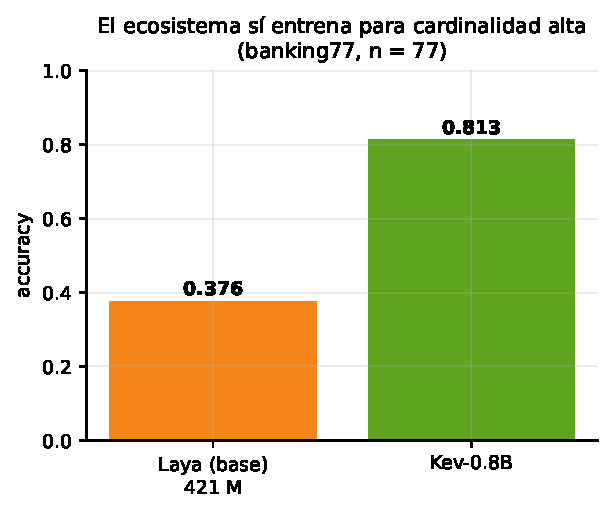
\includegraphics[width=\columnwidth]{fig7-accuracy-banking77}
\caption{Accuracy en \texttt{banking77} ($n = 77$) por configuración: Kev-0.8B (0.813) duplica al mejor
checkpoint de Laya (0.378) y triplica al checkpoint base (0.377). El ecosistema sí entrena para
cardinalidad alta, pero no todos los modelos por igual.}
\label{fig:accuracy-banking77}
\end{figure}

\subsection{El objeto de la tesis, en una cifra}

Sobre las \textbf{65\,185} distribuciones medidas (una fila por decisión), la diferencia entre la definición
de \texttt{confidence} más alta y la más baja de la \textbf{misma} distribución tiene:

\begin{table}[t]
\centering
\caption{Brecha interna de \texttt{confidence} sobre las 65\,185 distribuciones medidas: diferencia entre la
definición más alta y la más baja de una \emph{misma} distribución.}
\label{tab:brecha}
{\small
\setlength{\tabcolsep}{4pt}
\begin{tabular}{lr}
\toprule
estadístico & valor \\
\midrule
mediana & \textbf{0.288} \\
percentil 90 & \textbf{0.434} \\
máximo & \textbf{0.848} \\
\bottomrule
\end{tabular}}
\end{table}

Es decir: en el caso típico, dos implementaciones del mismo campo discrepan en casi tres décimas sobre el
mismo dato, y el peor caso llega a 0.85. Cualquier umbral fijado sobre una de las dos no significa lo mismo
sobre la otra.

\begin{figure}[t]
\centering
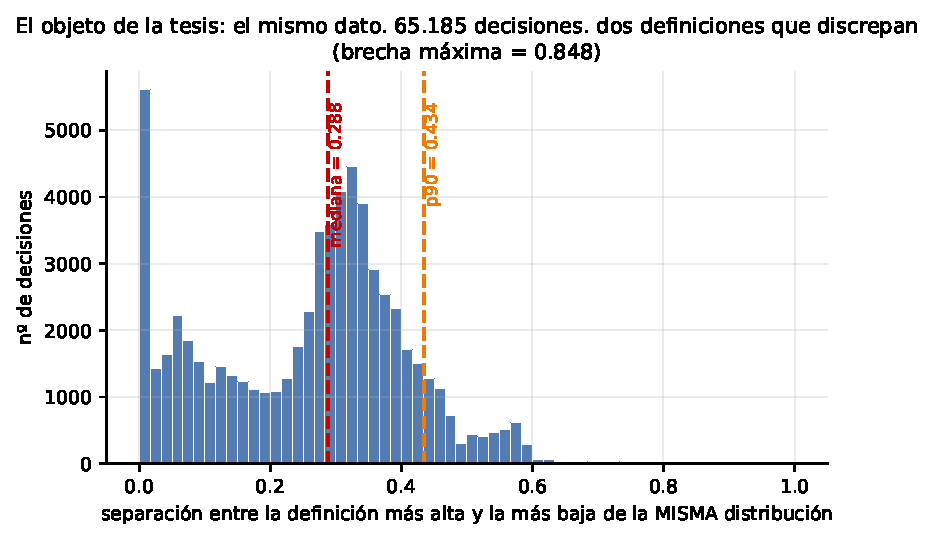
\includegraphics[width=\columnwidth]{fig1-brecha}
\caption{La cifra central: sobre las 65\,185 decisiones medidas, la definición más alta y la más baja de
\texttt{confidence} difieren con mediana 0.288 y alcance máximo 0.848. Un umbral fijado con una definición
no significa lo mismo con la otra.}
\label{fig:brecha}
\end{figure}

\subsection{El número no viaja; el mapa sí}

El titular es sobre el \textbf{nivel principal \texttt{raw}}, que es el que congela el pre-registro. En él,
de las 3\,564 celdas, \textbf{348 tienen mapa cerrado} entre definiciones (misma clase de equivalencia y
misma cardinalidad; 1\,044 si se cuentan los tres niveles), que son las únicas donde tiene sentido comparar
el porte directo contra el porte con mapa. El error absoluto medio:

\begin{table}[t]
\centering
\caption{Error absoluto medio del porte directo frente al porte con mapa, por subconjunto de celdas (nivel
\texttt{raw}). El porte directo se equivoca hasta dos órdenes de magnitud más que el porte con mapa.}
\label{tab:error-transferencia}
{\footnotesize
\setlength{\tabcolsep}{3pt}
\begin{tabular}{p{0.34\columnwidth}rlll}
\toprule
subconjunto & celdas & $\lvert\Delta\rvert$ directo & $\lvert\Delta\rvert$ con mapa & factor \\
\midrule
todas las celdas con mapa & 348 & 0.2528 & 0.0123 & 20.5$\times$ \\
\textbf{sin empates dominantes en el umbral} & \textbf{312} & \textbf{0.2337} & \textbf{0.0021} & \textbf{109.2$\times$} \\
solo modelos entrenados (sin control crudo) & 276 & 0.2289 & 0.0020 & 112.8$\times$ \\
solo $n = 2$ (Proposición 3) & 180 & 0.3006 & 0.0218 & 13.8$\times$ \\
solo $n \ge 3$ (Proposición 1) & 168 & 0.2015 & 0.0021 & 95.8$\times$ \\
nivel \texttt{L0} (debiasing sin etiquetas) & 324 & 0.2190 & 0.0059 & 37.1$\times$ \\
nivel \texttt{L1} (temperatura con etiquetas) & 312 & 0.3022 & 0.0024 & 126.0$\times$ \\
\bottomrule
\end{tabular}}
\end{table}

El porte directo se equivoca \textbf{del orden de cien veces más} que el porte con mapa. El matiz de la
tercera columna lo explica §5.4.

\begin{figure}[t]
\centering
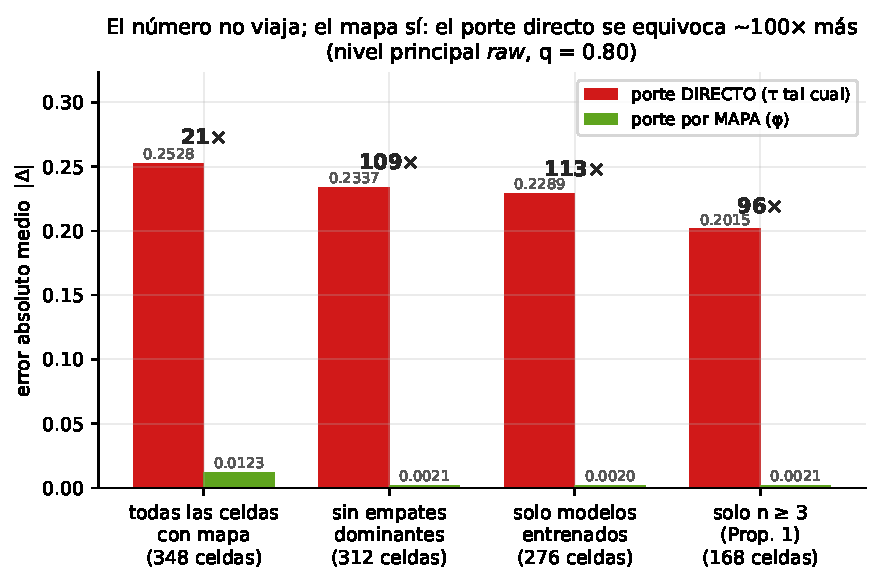
\includegraphics[width=\columnwidth]{fig2-directo-vs-mapa}
\caption{El titular: el porte directo del umbral (sin transformar) se equivoca del orden de cien veces más
que el porte con el mapa cerrado cuando este existe (0.2337 frente a 0.0021 sin empates dominantes).}
\label{fig:directo-vs-mapa}
\end{figure}

\textbf{Cómo leer la tabla.} El porte con mapa tiene un suelo que no es culpa del mapa: si el umbral cae
sobre un valor \textbf{empatado} en muchas salidas (modelos saturados), la cobertura salta y ni el mapa
puede dar $q$ exacto. Por eso la comparación limpia es la del subconjunto sin empates dominantes (masa por
debajo del 5\,\%), y por eso \texttt{delta\_mapa} debe leerse contra \texttt{delta} de la \textbf{misma}
celda, nunca como un cero absoluto. La columna \texttt{n\_empates\_tau} de la matriz declara, en cada celda,
cuántos ítems comparten el umbral.

\begin{figure}[t]
\centering
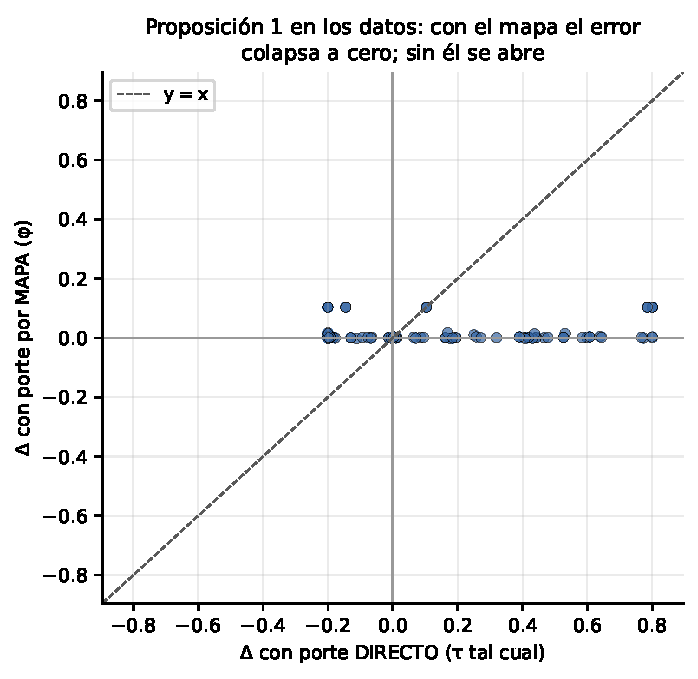
\includegraphics[width=\columnwidth]{fig3-delta-vs-mapa}
\caption{La Proposición 1 sobre los datos: celda a celda, la caída de cobertura del porte directo ($\lvert\Delta\rvert$ directo) contra la del porte con mapa. Con el mapa el error colapsa al suelo que imponen
los empates del umbral, no el mapa.}
\label{fig:delta-vs-mapa}
\end{figure}

\subsection{El promedio no es el resumen: la estructura está en el par}

La distribución de $\Delta$ es \textbf{bimodal}: hay pares de definiciones que coinciden y pares que fallan
en grande. El titular es el par, no la media global.

\begin{table}[t]
\centering
\caption{Caída de cobertura por par de definiciones (origen $A$ $\to$ destino $B$), ordenada por la mediana.
La mediana del par manda sobre la media global: el promedio engaña.}
\label{tab:par}
{\footnotesize
\setlength{\tabcolsep}{3pt}
\begin{tabular}{lrrrl}
\toprule
$A \to B$ & celdas & $\lvert\Delta\rvert$ mediana & $\lvert\Delta\rvert$ media & ¿mapa? \\
\midrule
\texttt{margin} $\to$ \texttt{jev} & 15 & \textbf{0.0023} & 0.0250 & sí \\
\texttt{jev} $\to$ \texttt{margin} & 15 & \textbf{0.0023} & 0.0293 & sí \\
\texttt{jev} $\to$ \texttt{pmax} & 99 & \textbf{0.0759} & 0.1568 & sí \\
\texttt{ent} $\to$ \texttt{jev} & 15 & \textbf{0.1837} & 0.1898 & sí \\
\texttt{ent} $\to$ \texttt{margin} & 15 & \textbf{0.1837} & 0.1898 & sí \\
\texttt{margin} $\to$ \texttt{pmax} & 15 & \textbf{0.2000} & 0.2253 & sí \\
\texttt{ent} $\to$ \texttt{pmax} & 15 & \textbf{0.2000} & 0.2421 & sí \\
\texttt{pmax} $\to$ \texttt{jev} & 99 & \textbf{0.2574} & 0.2973 & sí \\
\texttt{margin} $\to$ \texttt{ent} & 15 & \textbf{0.3474} & 0.3855 & sí \\
\texttt{jev} $\to$ \texttt{ent} & 15 & \textbf{0.3474} & 0.3857 & sí \\
\texttt{pmax} $\to$ \texttt{margin} & 15 & \textbf{0.5262} & 0.5154 & sí \\
\texttt{pmax} $\to$ \texttt{ent} & 15 & \textbf{0.7667} & 0.6787 & sí \\
\bottomrule
\end{tabular}}
\end{table}

Dos de las coincidencias son \textbf{identidades matemáticas}, no azar: (i) a $n = 2$, $C_{\text{Jev}}$ y
$C_{\text{mar}}$ son la \textbf{misma} función ($2\cdot p_{\max} - 1$), así que su porte directo ya da casi
cero; (ii) a cardinalidad alta, $C_{\text{Jev}} = (n\cdot p - 1)/(n - 1) \to p$, así que \texttt{jev} y
\texttt{pmax} convergen y sus umbrales casi coinciden. En el extremo opuesto,
$\text{pmax} \to \text{ent}$ es el peor par: no cambia la escala, cambia la \textbf{forma} de la función.

\begin{figure}[t]
\centering
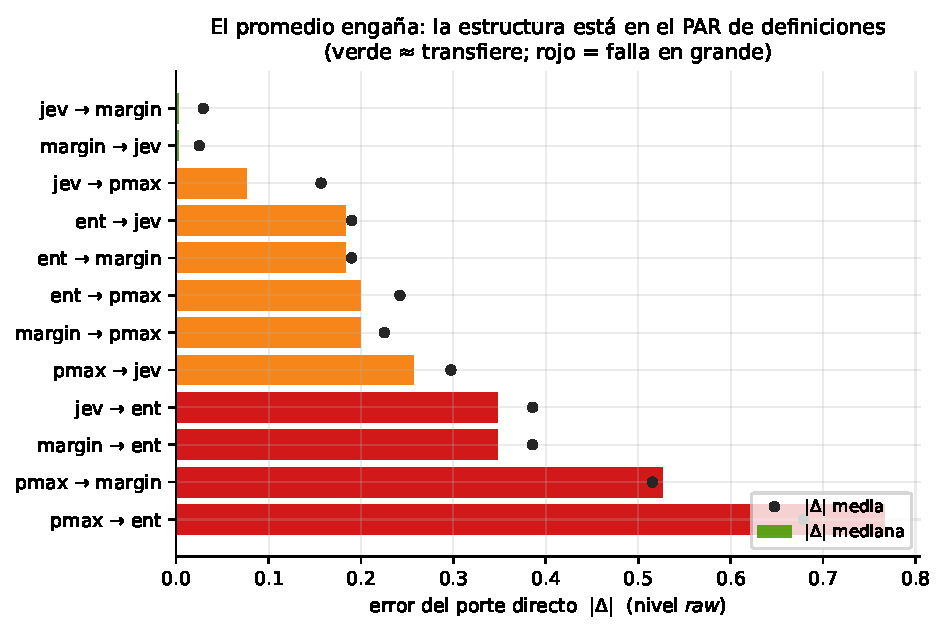
\includegraphics[width=\columnwidth]{fig4-por-par}
\caption{El promedio engaña: la estructura está en el par. Hay pares de definiciones que coinciden por
identidad matemática (medianas de 0.0023) y pares que fallan en grande (hasta 0.7667), y la media global
borra esa bimodalidad.}
\label{fig:por-par}
\end{figure}

Fracción de celdas que transfieren bien ($\lvert\Delta\rvert < 0.01$), por cardinalidad (nivel \texttt{raw}):

\begin{table}[t]
\centering
\caption{Fracción de celdas que transfieren bien ($\lvert\Delta\rvert < 0.01$) según la cardinalidad $n$. El
umbral solo viaja a cardinalidad alta.}
\label{tab:cardinalidad}
{\footnotesize
\setlength{\tabcolsep}{3pt}
\begin{tabular}{lrrl}
\toprule
$n$ & celdas con mapa & $\lvert\Delta\rvert$ mediana & \% con $\lvert\Delta\rvert < 0.01$ \\
\midrule
2 & 180 & 0.2141 & 14\,\% \\
3 & 30 & 0.1775 & 0\,\% \\
4 & 30 & 0.4085 & 0\,\% \\
5 & 60 & 0.2000 & 0\,\% \\
77 & 30 & 0.0058 & 63\,\% \\
151 & 18 & 0.0127 & 44\,\% \\
\bottomrule
\end{tabular}}
\end{table}

\begin{figure}[t]
\centering
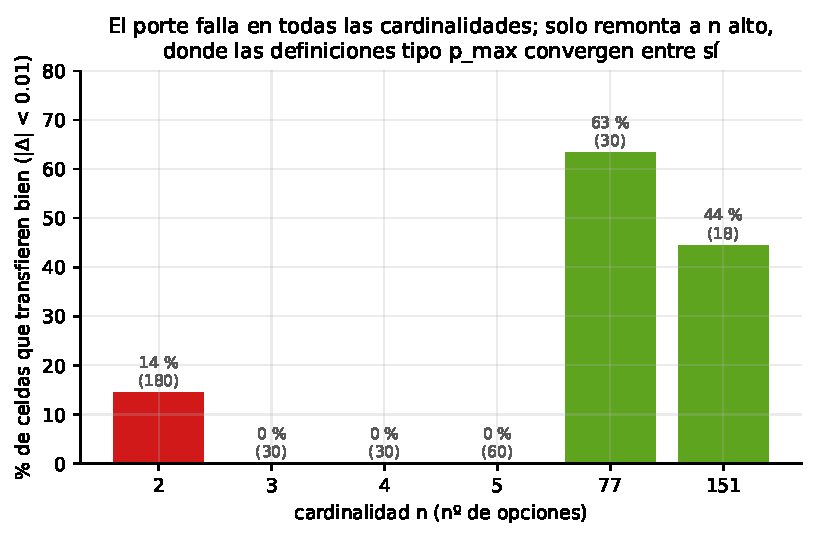
\includegraphics[width=\columnwidth]{fig5-por-cardinalidad}
\caption{Transferencia por cardinalidad $n$ (nivel \texttt{raw}): con $n \le 5$ casi ninguna celda
transfiere bien ($\lvert\Delta\rvert < 0.01$ en el 14\,\% de los casos y menos), mientras que a $n \ge 77$ la
mitad o más lo logra.}
\label{fig:por-cardinalidad}
\end{figure}

\subsection{Efecto de la cardinalidad}

\begin{table}[t]
\centering
\caption{Caída de cobertura y celdas significativas tras FDR, por cardinalidad $n$, con el dataset de
ejemplo. El porte falla en todas las cardinalidades.}
\label{tab:cardinalidad-fdr}
{\footnotesize
\setlength{\tabcolsep}{3pt}
\begin{tabular}{lrrrl}
\toprule
$n$ & celdas & $\lvert\Delta\rvert$ medio & celdas con FDR & dataset de ejemplo \\
\midrule
2 & 60 & 0.3042 & 52 & \texttt{typed-\allowbreak decisions} \\
3 & 60 & 0.2011 & 60 & \texttt{wanli} \\
4 & 60 & 0.3240 & 60 & \texttt{typed-\allowbreak decisions} \\
5 & 120 & 0.2664 & 119 & \texttt{sst5} \\
77 & 60 & 0.1638 & 52 & \texttt{banking77} \\
151 & 36 & 0.2140 & 32 & \texttt{clinc150} \\
\bottomrule
\end{tabular}}
\end{table}

El porte falla en todas las cardinalidades, pero con dos matices ya visibles en §5.4: a $n$ bajo el daño es
grande y sistemático, mientras que a cardinalidad alta ($n \ge 77$) las definiciones tipo $p_{\max}$
convergen entre sí y una parte de las celdas transfiere bien. La Proposición 3 predice que con $n = 2$ todas
las definiciones deberían ser equivalentes en orden; en los datos eso se cumple \textbf{dentro del par
$\text{jev} \leftrightarrow \text{margin}$} (misma función) y no en el resto, porque el porte directo cruza
escalas distintas aunque el orden sea el mismo. Es la distinción entre el número y el mapa.

\subsection{Dónde el umbral no viaja (nivel \texttt{raw}, $q = 0.80$, tras FDR)}

\begin{table}[t]
\centering
\caption{Celdas donde el umbral no viaja: nivel \texttt{raw}, $q = 0.80$, tras FDR. Portar el umbral pierde
toda la cobertura ($\Delta = 0.80$, cobertura B $= 0$) o casi toda.}
\label{tab:no-viaja}
{\footnotesize
\setlength{\tabcolsep}{3pt}
\resizebox{\columnwidth}{!}{%
\begin{tabular}{p{0.38\columnwidth}p{0.30\columnwidth}llrll}
\toprule
modelo & dataset & $n$ & $A \to B$ & $\Delta$ & IC95\,\% & cobertura B \\
\midrule
\texttt{Qwen/\allowbreak Qwen3.5-0.8B-Base} & \texttt{banking77} & 77 & \texttt{ent} $\to$ \texttt{margin} & 0.8000 & [0.800, 0.800] & 0.000 \\
\texttt{Qwen/\allowbreak Qwen3.5-0.8B-Base} & \texttt{sst5} & 5 & \texttt{pmax} $\to$ \texttt{ent} & 0.8000 & [0.800, 0.800] & 0.000 \\
\texttt{Qwen/\allowbreak Qwen3.5-0.8B-Base} & \texttt{typed-\allowbreak decisions} & 2 & \texttt{pmax} $\to$ \texttt{jev} & 0.8000 & [0.800, 0.800] & 0.000 \\
\texttt{Qwen/\allowbreak Qwen3.5-0.8B-Base} & \texttt{typed-\allowbreak decisions} & 2 & \texttt{pmax} $\to$ \texttt{ent} & 0.8000 & [0.800, 0.800] & 0.000 \\
\texttt{Qwen/\allowbreak Qwen3.5-0.8B-Base} & \texttt{typed-\allowbreak decisions} & 2 & \texttt{pmax} $\to$ \texttt{margin} & 0.8000 & [0.800, 0.800] & 0.000 \\
\texttt{convaiinnovations/\allowbreak laya/\allowbreak typed-decisions} & \texttt{typed-\allowbreak decisions} & 2 & \texttt{pmax} $\to$ \texttt{ent} & 0.8000 & [0.800, 0.800] & 0.000 \\
\texttt{jaredpalmer/\allowbreak kev-0.8b} & \texttt{typed-\allowbreak decisions} & 2 & \texttt{pmax} $\to$ \texttt{ent} & 0.8000 & [0.800, 0.800] & 0.000 \\
\texttt{Qwen/\allowbreak Qwen3.5-0.8B-Base} & \texttt{banking77} & 77 & \texttt{pmax} $\to$ \texttt{margin} & 0.7997 & [0.799, 0.800] & 0.000 \\
\texttt{Qwen/\allowbreak Qwen3.5-0.8B-Base} & \texttt{banking77} & 77 & \texttt{ent} $\to$ \texttt{jev} & 0.7997 & [0.799, 0.800] & 0.000 \\
\texttt{Qwen/\allowbreak Qwen3.5-0.8B-Base} & \texttt{banking77} & 77 & \texttt{jev} $\to$ \texttt{margin} & 0.7993 & [0.798, 0.800] & 0.001 \\
\texttt{Qwen/\allowbreak Qwen3.5-0.8B-Base} & \texttt{banking77} & 77 & \texttt{ent} $\to$ \texttt{pmax} & 0.7990 & [0.798, 0.800] & 0.001 \\
\texttt{Qwen/\allowbreak Qwen3.5-0.8B-Base} & \texttt{sst5} & 5 & \texttt{pmax} $\to$ \texttt{margin} & 0.7974 & [0.794, 0.800] & 0.003 \\
\bottomrule
\end{tabular}}}
\end{table}

La lectura es directa: hay celdas en las que portar el umbral \textbf{pierde toda la cobertura}. Quien
calibra al 80\,\% con una definición y despliega con otra puede terminar actuando en el 0\,\% de los casos
(o en todos), sin ningún aviso del modelo.

\begin{figure}[t]
\centering
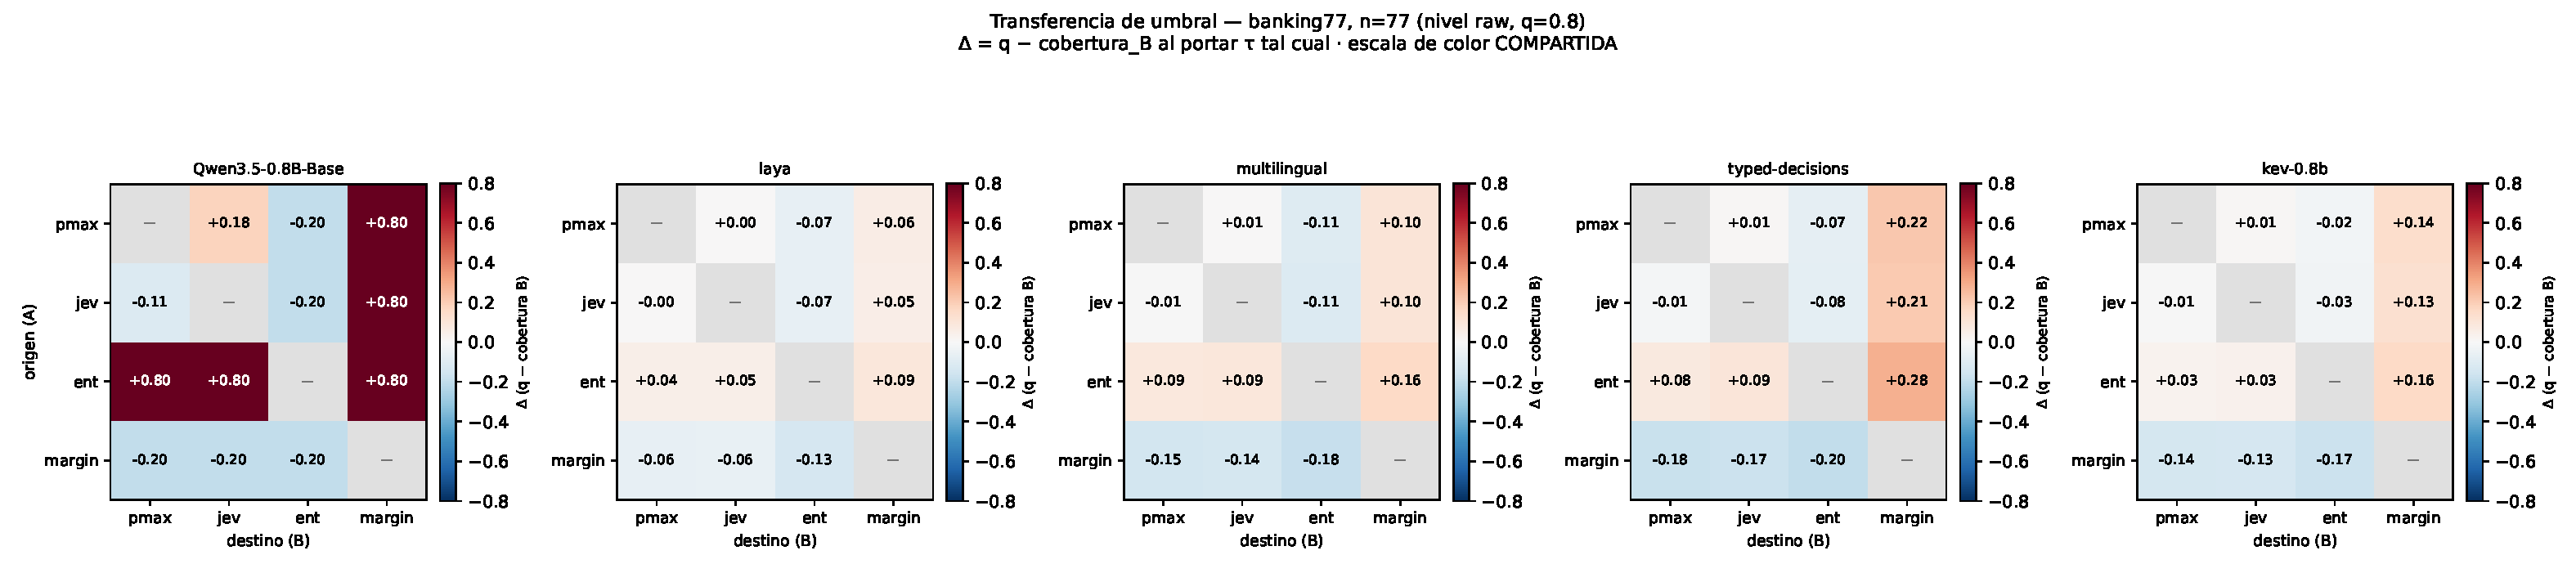
\includegraphics[width=\columnwidth]{fig8-heatmap-banking77}
\caption{Dónde el umbral no viaja: mapa de calor de la caída de cobertura en \texttt{banking77} ($n = 77$,
nivel \texttt{raw}), con filas de definición origen y columnas de definición destino. Cuando el modelo está
saturado, celdas enteras pierden toda la cobertura al cambiar de definición.}
\label{fig:heatmap-banking77}
\end{figure}

\subsection{Hallazgos de metrología del paso 0 (contexto)}

La corrida de verificación sobre \texttt{typed-decisions} dejó, además, dos resultados que no estaban en la
literatura del ecosistema y que son parte del instrumento:

\begin{enumerate}
\item \textbf{La \texttt{choice\_confidence} de Kev es la fórmula de Jev.}
   $(p_{\max} - 1/K)/(1 - 1/K) \equiv (K\cdot p_{\max} - 1)/(K - 1)$, verificado numéricamente para
   $K \in \{2,3,4,7,12\}$. Estaban registradas como definiciones distintas; por la Proposición 1, ese par
   transfiere el umbral de forma exacta.
\item \textbf{El campo \texttt{output\_tokens} tiene tres significados.} Jev y Laya lo reportan como 0 (no
   hay generación); Kev lo usa como recuento de tokens de la respuesta serializada (869\,310 en las mismas
   2\,000 decisiones). Es metrología del propio campo, no un fallo de Kev.
\end{enumerate}

Y sobre la misma corrida, el ECE cambia por completo según la definición: en \texttt{laya-typed-decisions}
va de \textbf{0.216} con $p_{\max}$ a \textbf{0.577} con la entropía normalizada, un factor
\textbf{2.7$\times$} sobre el mismo dato.

\begin{figure}[t]
\centering
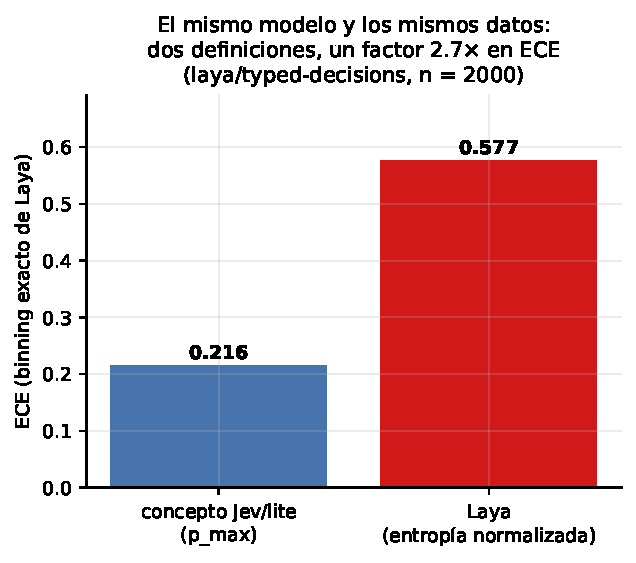
\includegraphics[width=\columnwidth]{fig6-ece-por-definicion}
\caption[El mismo ECE cambia con la definición de \texttt{confidence}]{El mismo dato, dos ECE: en
\texttt{laya-typed-decisions} el ECE va de 0.216 con $p_{\max}$ a 0.577
con la entropía normalizada, un factor 2.7$\times$. El ECE auto-reportado no es una propiedad del modelo
sino de la definición elegida.}
\label{fig:ece}
\end{figure}

\subsection{Extensiones declaradas (posteriores al pre-registro)}

Las cifras de las subsecciones anteriores están selladas por el pre-registro
\texttt{10.5281/zenodo.23266795}: \textbf{23 grupos, 65\,185 decisiones, 3\,564 celdas}. Las dos mediciones de
esta subsección son \textbf{posteriores} a ese pre-registro y se declaran aparte para no moverlas: no recalculan
la matriz sellada ni las filas crudas, se calculan como post-proceso sobre datos ya medidos o sobre un brazo
nuevo, y llevan su fecha.

\subsubsection{Quinta definición del campo: \texttt{conf\_score} (distancia al nivel modal)}

La documentación de TypeSafe define para la primitiva \texttt{score} una \texttt{confidence} que no estaba entre
las cuatro definiciones selladas:
\begin{equation}
\begin{aligned}
C_{\text{score}} &= \max\Bigl(0,\; 1 - \tfrac{1}{M}\,{\textstyle\sum_i}\, p_i\,\lvert i-m\rvert\Bigr),\\
M &= \tfrac{1}{n}\,{\textstyle\sum_i}\, \bigl\lvert i-\tfrac{n-1}{2}\bigr\rvert ,
\end{aligned}
\end{equation}
donde $M$ es la desviación absoluta media de la rejilla uniforme (\emph{MAD} uniforme) y $m$ el nivel modal.
No es una variante de $C_{\text{jev}}$: $C_{\text{jev}}$ mide \textbf{concentración en el máximo};
$C_{\text{score}}$ mide \textbf{dispersión alrededor del nivel modal}. Dos distribuciones con el mismo $p_{\max}$
dan valores distintos. Y es \textbf{ordinal}: exige que los niveles tengan orden y distancia, así que solo se
mide donde el orden existe.

\begin{table}[t]
\centering
\caption{La quinta definición sobre \texttt{sst5} (5 niveles ordinales, 5 configuraciones, 5\,505 decisiones).
La brecha es la diferencia entre la definición más alta y la más baja de la \emph{misma} distribución; el ECE se
calcula sobre la misma corrida y la misma etiqueta de corrección que las otras cuatro.}
\label{tab:extension-score}
{\footnotesize
\begin{tabular}{@{}lr@{}}
\toprule
Brecha, mediana con 4 definiciones & 0.272 \\
Brecha, mediana con 5 definiciones & \textbf{0.290} (p90 0.411, máx 0.581) \\
\midrule
ECE global, $C_{\text{pmax}}$ & 0.204 \\
ECE global, $C_{\text{jev}}$ & 0.184 \\
ECE global, $C_{\text{ent}}$ & 0.199 \\
ECE global, $C_{\text{mar}}$ & 0.237 \\
ECE global, $C_{\text{score}}$ & \textbf{0.241} \\
\midrule
Verificación contra el servicio real & $\lvert\Delta\rvert \le 0.0050$ en 800 filas \\
\bottomrule
\end{tabular}}
\end{table}

\textbf{Por qué solo \texttt{sst5}.} En \texttt{banking77} (77), \texttt{clinc150} (151) y
\texttt{typed-decisions} (2, 4, 5) las etiquetas son nominales: el índice $i$ no significa nada y usarlo sería
añadir un supuesto, no medir. En \texttt{wanli} (3) el orden es discutible. Se declara el límite en lugar de
inventar la escala.

\textbf{El hallazgo que añade.} La quinta definición \textbf{no tiene un sesgo estable}: es la más baja de las
cinco en el \textbf{70.3\,\%} de las filas del control crudo Qwen y la más alta en el \textbf{92.6\,\%} de las de
Laya-multilingual. El signo de la discrepancia depende del modelo, no de la definición --- que es exactamente el
objeto de este trabajo, ahora con una definición más en la lista.

\subsubsection{Brazo pagado: el modelo detrás del campo}

Hasta aquí todo se midió sobre pesos abiertos. El servicio real de TypeSafe (\texttt{jev-1.13.0}, una petición
por ítem) se midió sobre los mismos cinco datasets y se publica como brazo aparte: \textbf{14\,277 decisiones},
gasto \textbf{USD 0.79}, con \texttt{probabilities} y \texttt{confidence} redondeadas a \textbf{0.01} por el
servicio.

\begin{table}[t]
\centering
\caption{Brazo pagado: el servicio real sobre los cinco datasets etiquetados. La última columna es el contador
\texttt{output\_tokens} que reporta el servicio; en todos los brazos de pesos abiertos ese mismo contador vale
cero.}
\label{tab:brazo-pagado}
{\footnotesize
\setlength{\tabcolsep}{4pt}
\begin{tabular}{@{}lrrrr@{}}
\toprule
dataset & $n$ & ítems & accuracy & tokens de salida \\
\midrule
\texttt{banking77} & 77 & 3\,076 & 0.796 & 2\,547\,728 \\
\texttt{clinc150} & 151 & 3\,100 & 0.901 & 4\,034\,486 \\
\texttt{sst5} & 5 & 1\,101 & 0.541 & 19\,818 \\
\texttt{typed-decisions} & 2, 4, 5 & 2\,000 & 0.733 & 270\,290 \\
\texttt{wanli} & 3 & 5\,000 & 0.754 & 220\,650 \\
\bottomrule
\end{tabular}}
\end{table}

Dos observaciones de metrología del propio campo. (i) El contador \texttt{output\_tokens} \textbf{no es cero} en
el servicio (7\,092\,972 en total), a diferencia de los brazos de pesos abiertos: el campo \emph{tokens de
salida} no distingue por sí solo un modelo de decisión de uno generativo; esa lectura solo vale donde se controla
la implementación. (ii) La confianza que el servicio \textbf{devuelve} coincide con la definición que la
especificación le asigna a cada primitiva: $C_{\text{score}}$ en las filas \texttt{score} ($\lvert\Delta\rvert
\le 0.0050$ sobre 800 filas) y $C_{\text{jev}}$ en las de \texttt{choice} (600 filas). La especificación describe
el servicio real, no una reconstrucción.

Sumado a los brazos abiertos, el conjunto tiene \textbf{79\,462 decisiones} y una brecha mediana de
\textbf{0.273} (p90 0.435) --- el mismo orden que la cifra sellada de 0.288, ahora con seis modelos.

\textbf{El porte del umbral con la rejilla de 0.01.} Error absoluto medio del porte sobre las celdas con mapa
cerrado (nivel \texttt{raw}, las tres $q$; 420 celdas):

\begin{table}[t]
\centering
\caption{Porte del umbral en el conjunto combinado, por modelo. La última columna es la fracción media de ítems de
prueba que comparten el umbral (empates inducidos por la rejilla de 0.01 del servicio).}
\label{tab:porte-pagado}
{\footnotesize
\setlength{\tabcolsep}{3pt}
\resizebox{\columnwidth}{!}{%
\begin{tabular}{@{}lrrrr@{}}
\toprule
modelo & celdas & $\lvert\Delta\rvert$ directo & $\lvert\Delta\rvert$ con mapa & factor \\
\midrule
\texttt{typesafe-ai/jev} & 72 & 0.1735 & \textbf{0.0130} & 13.4$\times$ \\
\texttt{laya/multilingual} & 72 & \textbf{0.1315} & 0.0018 & 75.1$\times$ \\
\texttt{laya} & 66 & 0.2581 & 0.0028 & 91.7$\times$ \\
\texttt{laya/typed-decisions} & 72 & 0.2515 & 0.0014 & 174.4$\times$ \\
\texttt{kev-0.8b} & 66 & 0.2813 & 0.0022 & 128.5$\times$ \\
\texttt{Qwen3.5-0.8B} (control) & 72 & 0.3441 & 0.0517 & 6.7$\times$ \\
\midrule
global & 420 & 0.2392 & 0.0124 & 19.3$\times$ \\
\bottomrule
\end{tabular}}}
\end{table}

La lectura es en dos partes, y la segunda corrige la intuición. (i) El porte \textbf{directo} de Jev (0.1735) es
de los mejores, pero \textbf{no el mejor}: el checkpoint \texttt{laya/multilingual} transfiere mejor (0.1315) sin
ser el modelo de referencia del campo. Comparar $\lvert\Delta\rvert$ directo entre modelos mezcla dos causas ---la
definición y la calidad del modelo--- y por eso el titular de este trabajo es el par de definiciones, no el
modelo. (ii) El porte \textbf{con mapa} de Jev es \textbf{4.6 a 9.3 veces} el de los checkpoints abiertos (0.0130
frente a 0.0014--0.0028) y su factor directo/mapa es \textbf{13.4$\times$}, un orden de magnitud menor que el de
ellos (75--174$\times$). La causa está medida: la rejilla de 0.01 reasigna masa a valores empatados y
\textbf{2.5\,\%} de los ítems de prueba de Jev comparten el umbral, frente a \textbf{0.1\,\%} en los abiertos
(25$\times$), con 4 de 72 celdas por encima del 5\,\% de empate frente a 0 en las abiertas. El mapa cerrado sigue
siendo válido (Proposición~1); lo que la rejilla degrada es la \textbf{resolución del umbral}, no la equivalencia
entre definiciones.

\emph{Fuentes:} \path{results/matrix/EXTENSION_CONF_SCORE.md} y
\path{results/matrix_pagado/RESUMEN_MATRIZ_PAGADO.md}; se regeneran con
\path{src/matriz/extension_conf_score.py} y \path{src/matriz/correr_matriz_pagado.sh}. Ninguna de estas dos
extensiones modifica el nivel \texttt{raw} sellado, ni las 3\,564 celdas, ni las 65\,185 filas crudas.

\section{Discusión}
\label{sec:discusion}

\subsection{El hallazgo tiene dos capas}

El resultado principal es que un umbral de \texttt{confidence} no transfiere entre implementaciones y que el
promedio no describe el fenómeno. Al mirar celda a celda aparecen dos capas distintas, y confundirlas lleva a conclusiones opuestas (documentado en \texttt{docs/erratas\_especificacion.md}, E2).

\textbf{Capa 1, la escala.} Dos definiciones pueden ordenar las decisiones igual y aun así estar en escalas distintas. $C_{\max}=p$ y $C_{\mathrm{Jev}}=(n\cdot p-1)/(n-1)$ inducen el mismo umbral en orden, de modo que existe un mapa cerrado $\psi=\phi^{-1}$ entre ellas. El número no viaja ($|\Delta|$ mediano de 0.076 en un sentido del par \texttt{pmax} $\leftrightarrow$ \texttt{jev} y 0.257 en el otro, nivel \texttt{raw}), pero el mapa sí transfiere (0.0013 de mediana, 0.0049 de media): la escala se corrige, la cifra no sirve tal cual.

\textbf{Capa 2, la forma.} Entre definiciones de clases distintas ($p_{\max}$, entropía, margen) no existe ni número ni mapa. \texttt{pmax} $\to$ \texttt{ent} tiene mediana de 0.77: es el caso en que la confianza «alta» de una definición y la de la otra ordenan las decisiones de forma diferente, no solo con otra escala. Aquí no hay nada que traducir y el porte directo es lisa y llanamente una extrapolación inválida.

La coexistencia de las dos capas es la razón de que el resultado no se pueda resumir con una media: la misma tabla contiene identidades exactas (14\,\% de las celdas con $n=2$ transfieren bien) y desastres (celdas con $\Delta=0.80$ y cobertura 0).

\subsection{Por qué el orden se preserva y el número no}

Sea $f$ una transformación creciente de $p_{\max}$. Un umbral $\tau$ sobre $f(p_{\max})$ selecciona el mismo conjunto de decisiones que el umbral $f^{-1}(\tau)$ sobre $p_{\max}$, porque $f$ monótona no cambia el orden. Por eso $C_{\mathrm{Jev}}$ y $C_{\max}$ (fijado $n$) seleccionan lo mismo con el umbral traducido; $C_{\mathrm{mar}}$ también, pero \textbf{solo a $n = 2$}, donde vale $2\cdot p_{\max}-1$: a $n \ge 3$ el margen depende de las dos probabilidades mayores y no es función de $p_{\max}$. Pero el valor de $f$ depende de $n$ y de la definición, así que la misma cifra $0.7$ significa coberturas distintas. Y cuando $f$ deja de ser una función de $p_{\max}$ (la entropía usa toda la distribución, no solo el máximo), ni siquiera existe el mapa.

Esto es exactamente lo que predice la Proposición 1 y lo que mide el factor 109$\times$: el costo de confundir «mismo orden» con «mismo número».

\subsection{El umbral es una política, no un número suelto}

En un sistema que decide, el umbral no es un parámetro cosmético: define cuándo el modelo actúa y cuándo se abstiene. Un umbral trasladado sin mapa no solo cambia una métrica de calibración, cambia la política de abstención. Las celdas de \S5.6 lo muestran en su forma extrema: con $q=0.80$ puede terminar actuando en el 0\,\% de los casos. Para quien integra un modelo tipo Jev, la conclusión práctica es que el campo \texttt{confidence} no es un contrato entre implementaciones: es un número local, válido dentro de la definición que lo produjo.

Y sin embargo el ecosistema lo trata como si lo fuera. La revisión de implementaciones (Kev, Laya, AnyJev, open-decision-ai) muestra que cada una publica su fórmula bajo el mismo nombre y que ninguna documenta la relación con las demás. Ese vacío es el que este instrumento llena: no descubre que hay sobre-confianza (eso ya se midió puertas adentro de varias implementaciones), sino que cuantifica el error de trasladar el umbral entre ellas y entrega el mapa cuando existe.

\subsection{Calibración de las implementaciones medidas}

La literatura reciente mide la calibración dentro de una definición (por ejemplo, ECE de Laya tal como se distribuye). Este trabajo mide entre definiciones, que es una pregunta distinta y hasta ahora sin tabla. Los dos resultados no se contradicen: un modelo puede estar bien calibrado respecto de su propia definición y aun así ser inutilizable como fuente de umbral para otra. La cifra de \S5.7 (el ECE cambia 2.7$\times$ según la definición, sobre el mismo dato) ilustra que buena parte de las discrepancias que se atribuyen al modelo son, en realidad, discrepancias del medidor.

\subsection{Limitaciones}

\begin{itemize}
\item Cobertura de modelos. Cinco configuraciones de hasta 0.8B, todas las que caben en 6 GB. Los modelos de 4B a 9B del ecosistema quedan como extensión declarada.
\item Dos grupos ausentes. \texttt{clinc150} en el checkpoint base de Laya (ventana de 512 tokens, 126 de 151 opciones) y \texttt{kev-suites} (no carga en el Hub). Ninguno altera las conclusiones, pero acotan el alcance medido a 23 de 25 combinaciones.
\item El mapa existe dentro de clases y a cardinalidad fija. Las celdas sin mapa (2\,520 de 3\,564) no son «fallos»: son el resultado de que no haya traducción matemática posible. La matriz las marca como tales.
\item El control crudo infla el porte directo en las celdas con empates de umbral (modelo sin entrenar, salidas saturadas). Por eso la comparación limpia excluye las celdas dominadas por empates y la de referencia es la de 312 celdas (109$\times$, nivel \texttt{raw}).
\item Las definiciones opacas (\texttt{act\_probability}, \texttt{open-decision-ai}) quedaron fuera de la matriz por decisión de alcance, ya que no son funciones de la distribución.
\end{itemize}

\subsection{Relación con los trabajos previos}

Este resultado es un instrumento, y se sostiene aunque otro publique un hallazgo cercano. La calibración de un modelo puntual (por ejemplo, la medición de Laya tal cual se distribuye) es un hallazgo fechado; la matriz de transferencia y la librería que la reproduce son infraestructura. El instrumento no compite con esa literatura: la cita, la usa como punto de partida y la extiende al eje que le faltaba, el eje entre definiciones.

Las demás aristas del eje (por qué el término de RL no induce calibración, la ablación del objetivo de entrenamiento, la cartografía del ecosistema, la coherencia frente a la negación) están ocupadas por trabajos recientes y quedan fuera de esta tesis. Aquí lo medido es, deliberadamente, el hueco que quedaba abierto: la transferencia de umbrales entre definiciones incompatibles del mismo campo.

\section{Conclusión y artefactos}
\label{sec:conclusion}

\subsection{Conclusión}

El ecosistema abierto de modelos de decisión tipo Jev comparte un nombre de campo, \texttt{confidence}, y una promesa: que sirve para fijar un umbral de actuación. La medición sobre \textbf{23 grupos, 65\,185 decisiones y 3\,564 celdas} muestra que esa promesa \textbf{no viaja entre implementaciones}. Sobre la \textbf{misma} distribución, la definición de \texttt{confidence} más alta y la más baja difieren con mediana \textbf{0.288} y máximo \textbf{0.848}. Portar el umbral tal cual (copiar la cifra) se equivoca del orden de \textbf{cien veces} más que portarlo con el mapa matemático cuando este existe (0.2337 contra 0.0021, sobre las 312 celdas del nivel principal \texttt{raw} sin empates dominantes). Y en las celdas de peor caso, el porte directo pierde \textbf{toda} la cobertura: quien calibra al 80\,\% con una definición puede terminar actuando en el 0\,\% con otra.

El resultado tiene dos capas. La \textbf{escala} hace que el número no viaje aunque el orden se preserve; la \textbf{forma} hace que entre clases de definiciones distintas no exista ni número ni mapa. Dos pares que se creían distintos resultan ser la \textbf{misma} fórmula (la \texttt{choice\_confidence} de Kev es la de Jev; con $n=2$, $C_{\mathrm{Jev}}$ y el margen coinciden), lo que da transferencia exacta donde otros ven incompatibilidad.

El aporte no es el hallazgo de que las implementaciones discrepan, que era de esperar. El aporte es el \textbf{instrumento} que permite cuantificar y corregir esa discrepancia, y que sigue valiendo aunque cada premisa particular se cierre.

\subsection{Artefactos entregados}

\begin{table}[htbp]
\centering
\caption{Artefactos entregados}
\label{tab:artefactos}
\small
\begin{tabular}{@{}c >{\raggedright\arraybackslash}p{4.9cm} >{\raggedright\arraybackslash}p{2.3cm}@{}}
\toprule
\# & Artefacto (y dónde vive) & Estado \\
\midrule
1 & Especificación formal de las definiciones (DEF-1..DEF-8, Proposiciones 1 a 3) y erratas, en \path{paper/03_especificacion_confidence.md} & hecho \\
2 & Librería \texttt{jev-conf-metrics}, en \path{src/jev_conf_metrics/} & hecho (67 tests) \\
3 & Arnés de conformidad (tests T1..T8), en \path{tests/} & hecho \\
4 & Matriz de transferencia de umbrales, en \path{results/matrix/matriz_transferencia.csv} & medida (3\,564 celdas) \\
5 & Dataset de mediciones crudas, en \path{results/crudos/}, con \texttt{row\_hash} por fila & medido (65\,185 filas) \\
6 & Scripts regeneradores, en \path{src/matriz/} & hechos \\
7 & Figuras (mapas de calor por dataset y cardinalidad), en \path{paper/figures/} & hechas \\
8 & Pre-registro con DOI, en \path{paper/04_pre_registro.md} $\to$ Zenodo & publicado (\path{10.5281/zenodo.23266795}) \\
9 & Repositorio \path{github.com/Arbues/tesis1-jev-confidence} & \textbf{público} (Apache-2.0 / CC-BY-4.0) \\
10 & Extensión declarada: quinta definición del campo (\texttt{conf\_score}), en \path{results/matrix/EXTENSION_CONF_SCORE.md} & medida (5\,505 decisiones) \\
11 & Extensión declarada: brazo pagado (API real \texttt{jev-1.13.0}), en \path{results/pagado/} & medido (14\,277 decisiones) \\
\bottomrule
\end{tabular}
\end{table}

Todo el conjunto se regenera con \texttt{python -m pytest tests/ -q} seguido de los tres scripts de \texttt{src/matriz/} (\S4.5). Ninguna cifra del paper se escribe a mano: todas provienen del informe regenerable.

\subsection{Trabajo futuro}

El arco completo tiene tres etapas, y esta tesis cubre la primera.

\begin{itemize}
\item \textbf{Tesis 1 (este trabajo, medida).} El instrumento: medir y cuantificar la transferencia de umbrales entre las definiciones incompatibles del campo \texttt{confidence}.
\item \textbf{Tesis 2 (mecanismo).} Una vez medido el problema, inducir calibración en el objetivo de entrenamiento, no solo por ajuste post-hoc. La pregunta heredada es por qué el término de RL de RLCD no bastó, que la literatura reciente ya exploró y que aquí se da por ocupada.
\item \textbf{Taller de Tesis (teoría).} Las condiciones necesarias y suficientes para que una regla de puntuación estrictamente propia induzca un umbral que viaje entre definiciones.
\end{itemize}

Extensiones inmediatas del instrumento: medir los modelos de 4B a 9B en el Mac Mini, incorporar las definiciones opacas cuando exista una forma de tratarlas, y repetir la matriz cuando aparezcan nuevas implementaciones (el instrumento está diseñado para eso, no para un conjunto fijo de modelos).

\subsection{Disponibilidad}

Repositorio \textbf{público} \url{github.com/Arbues/tesis1-jev-confidence} (Apache-2.0 el código, CC-BY-4.0 el paper y la documentación). El pre-registro con el diseño congelado tiene DOI \textbf{10.5281/zenodo.23266795}.


\bibliographystyle{IEEEtran}
\bibliography{referencias}

\end{document}
